\vspace{1.0cm}
\section{Model and Estimation}
\subsection{Model Construction}
\subsubsection{Wait Time and Waiting Passengers}

\hspace{0.5cm} I first construct a model to specify the relationship between unobservable wait time and also the unobservable number of waiting passengers from the equilibrium data. This approach is similar to that of Frechette et al. (2016). There are I locations:\{1,...,I\} in Manhattan, and each day is divided into hours. Hereafter I reserve i and j for locations, k and l for areas (defined later), and h for hours. From the number of medallions in Manhattan at location i at hour h ($N_{ih}$), the number of trips which depart from location i at hour h ($T_{ih}$) and average time (minutes) of trips whose pickup location is i and hour is h ($m_{ih}$), the fraction of vacant taxis at location i at hour h is calculated as $1-\frac{T_{ih}m_{ih}}{60N_{ih}}$. I first set the whole number of medallions in Manhattan $N_h$ and assign each location the number of medallions depending on the trips completed in each location. I use the number of medallions which picked up, not dropped off, passengers at location i at hour h to allocate $N_h$ to each location i to obtain $N_{ih}$, because I don't specify how each driver acts after he/she dropped his/her passengers off.\footnote{Estimation exercised later shows that search time is long enough for some drivers to move to other locations to increase the probability of pickup. There are gaps between the number of pickups and dropoffs at each location and it's almost obvious that some drivers move to other locations after dropoff. According to Buchholz (2016), Pr(picking new passengers up at location i $|$ dropping previous passengers off at location i) is between 0.4 and 0.5, though the definitions of locations and hours are a bit different.} I also assume the number of medallions $N_{ih}$ to be exogenously determined conditional on location and time, and thus search time at location i at hour h ($s_{ih}$) is not affected by individual drivers' labor supply decision. I justify this assumption considering that drivers with leased cars, which consist of most of the medallions, had to drive at least 9 hours within 12-hour shift until 2015, and thus not so flexible to start or quit driving depending on the market conditions, especially during peak times. Moreover, demand can often be predicted (so drivers can react to it reasonably) and highly correlated with hours and locations which I control.\footnote{I concisely analyze the supply side with TLC data and show some evidence of inflexible labor supply in Appendix A.} From these numbers, $s_{ih}$ is readily obtained, $s_{ih} = \frac{60N_{ih}}{T_{ih}}-m_{ih}$. 

Next, let the total length of road at location i, $L_i$, then there are $\frac{N_{ih}}{L_i}$ cabs per mile at location i. If cabs are uniformly distributed within the same location i, then there are $\frac{N_{ih}}{L_i}(1-\frac{T_{ih}m_{ih}}{60N_{ih}})$ vacant taxis every mile (A). Lastly, let $v_{ih}$ be average velocity (mph), then it takes $\frac{60}{v_{ih}}$ minutes for each cab to move one mile (B). If passengers appear randomly within location i, then the wait time at location i at hour h ($w_{ih}$) for those passengers is calculated\footnote{There would be some passengers who could get on yellow cabs just after they appeared and oppositely other people who saw that vacant cabs just passed by, and thus wait time distributes between 0 and $\frac{B}{A}$, so wait time on average would be $\frac{B}{2A}$. But as I don't consider other hindrances when looking for vacant cabs (e.g. there are many traffic lines so that passengers can't get on some vacant cabs), I use $\frac{B}{A}$ instead of $\frac{B}{2A}$.} by $\frac{B}{A}$ and thus, $\frac{60}{\frac{v_{ih}}{L_i}(N_{ih}-\frac{T_{ih}m_{ih}}{60})}$. A simple example is sketched in Figure \ref{fig:taxi_picture}. $L_i$ is by construction exogenous and I assume that $m_{ih}$ and $v_{ih}$ are also exogenous.

\begin{figure}[h]
\begin{center}
\caption{Schematic of Location i}\label{fig:taxi_picture}\\
\end{center}
{\footnotesize \noindent If the average velocity is 12 mph and the number of vacant cabs per mile is 2 as in the image at location i at hour h, then wait time is calculated as $\frac{5}{2}$=2.5 minutes.}
\begin{center}
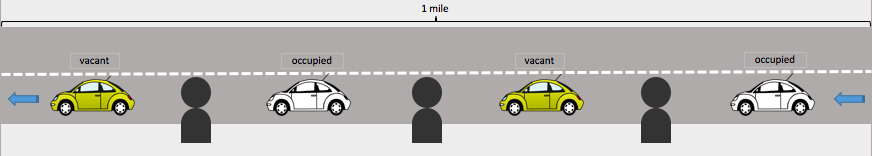
\includegraphics[width=16.5cm]{Figures/taxi_picture.png}
\end{center}
\end{figure}

Furthermore, I relate the equilibrium number of trips ($T_{ih}$) to the proxy for the number of waiting passengers at location i at hour h ($Q^d_{ih}$) without any other endogenous variables. I set $Q^d_{ih}$ as in Equation (\ref{eq:Q^d}) below, where $v^H$ is the fastest velocity in Manhattan for each day. This comes from the simple idea that as the number of cabs per mile is higher and as the velocity is closer to the maximum, the gap between the number of waiting passengers and those who got on taxis would be smaller. I also set $P_{ij}$ the price or fare of trips from location i to j in dollars, and $\delta_{ij}$ the distance between the two locations in miles for later use.

The equations of wait time (reprint) and proxy for the number of waiting passengers at location i at hour h are as follows. I omitted search time because it does not directly enter in the demand curve specified below. The variables discussed are summarized in Table \ref{tab:summary_variables}.

\begin{equation}
w_{ih} = \frac{60}{\frac{v_{ih}}{L_i}(N_{ih}-\frac{T_{ih}m_{ih}}{60})}\label{eq:w}
\end{equation}

\begin{equation}
Q^d_{ih} = T_{ih}\{1+\frac{L_i}{N_{ih}}(\frac{1}{v_{ih}}-\frac{1}{v^H})\}\label{eq:Q^d}
\end{equation}

\noindent From these two equations, the relationship between wait time and waiting passengers is

\begin{equation}
w_{ih} = \frac{3600L_i}{v_{ih}(60N_{ih}-\frac{m_{ih}Q^d_{ih}}{1+\alpha_{ih}})}\label{eq:w_Q^d}
\end{equation}
where $\alpha_{ih}$ = $\frac{L_i}{N_{ih}}(\frac{1}{v_{ih}}-\frac{1}{v^H})$

\begin{table}[h]
\caption{Summary of the Variables Used in the Model}\label{tab:summary_variables}\\

{
\def\sym#1{\ifmmode^{#1}\else\(^{#1}\)\fi}
\begin{center}
\begin{tabular}{l*{5}{l}}
\hline\hline
Variable & \multicolumn{1}{c}{Meaning}\\
\hline
 \multicolumn{1}{c}{$N_{ih}$} & Number of Medallions at Location i at Hour h\\
 \multicolumn{1}{c}{$T_{ih}$} & Number of Trips Departing from Location i at Hour h\\
 \multicolumn{1}{c}{$m_{ih}$} & Time of Trips Departing from Location i at Hour h (min.)\\
 \multicolumn{1}{c}{$L_i$} & Road Length at Location i (mile)\\
 \multicolumn{1}{c}{$v_{ih}$} & Velocity of Cabs at Location i at Hour h (mph)\\
 \multicolumn{1}{c}{$v^H$} & Fastest Velocity in the Day (mph)\\
 \multicolumn{1}{c}{$s_{ih}$} & Search Time at Location i at Hour h (min.)\\
 \multicolumn{1}{c}{$w_{ih}$} & (Unobservable) Wait Time at Location i at Hour h (min.)\\
 \multicolumn{1}{c}{$Q^d_{ih}$} & (Unobservable) Number of Waiting Passengers at Location i at Hour h\\
  \multicolumn{1}{c}{$P_{ij}$} & Price of Trips from Location i to j (dollar)\\
 \multicolumn{1}{c}{$\delta_{ij}$} & Distance between Location i to j (mile)\\

 


\hline\hline
\end{tabular}
\end{center}
}


\end{table}


\vspace{0.5cm}

\subsubsection{Demand Curve}

\hspace{0.5cm} Using the relationship built above, I specify the demand curve as in Equation (\ref{eq:demand_curve}). By this functional form, I assume that the elasticities of demand with respect to price and wait time to be constant. This assumption is relaxed later when I introduce cross terms of those with dummy variables of pickup/dropoff locations. While Frechette et al. (2016) use demand curve with no identification of locations,  Buchholz (2016) adopts the curve with time, origin and destination with fixed labor supply, so in that sense, my estimation is similar to that of Buchholz (2016). 


\begin{equation}
 log (Q^d_{ijh}) = \beta_0 + \beta_1 log (P_{ij}) + \beta_2 log (w_{ih}) + \mathbf{\bm{\gamma} X_{ijh}} + \epsilon_{ijh} \label{eq:demand_curve}
\end{equation}

\indent The number of waiting passengers at location i who is heading for location j is just a fraction of the number of trips from location i to j to that of trips where the origin is location i:   $Q^d_{ijh}$ = $\frac{T_{ijh}}{T_{ih}}Q^d_{ih}$. Log is natural logarithm, $P_{ij}$ is the price from location i to j as defined above, $w_{ih}$ is wait time for passengers at location i at hour h, and $\mathbf{X_{ijh}}$ is a vector containing other exogenous demand shifters. Importantly, the fare increased in September 2012, so there is a variation of $P_{ij}$.

$\epsilon_{ijh}$ is an error term which is assumed to be independent and identically distributed except for wait time, and this is a crucial assumption to estimate the elasticities without bias. $\epsilon_{ijh}$ contains any variables which are not observable or observed but not included in the model, such as income of residents at location i/j or the characteristics of location i/j. I justify the assumption as the following reasoning. Regarding $P_{ij}$, it is determined outside market by TLC and though passengers can choose from where to where to go, $Q^d_{ijh}$ would not be affected by $P_{mn}$, as $Q^d_{ijh}$ is not the same as $Q^d_{mnh}$ even if distance $\delta_{ij}$ and $\delta_{mn}$ are the same (in other words, they are not substitutes each other). As I set locations small enough so that there would be few variations of price within $P_{ij}$, $\epsilon_{ijh}$ would not be correlated with $P_{ij}$, though each location has some fixed effects.

With respect to $w_{ih}$, as it is surely correlated with $\epsilon_{ijh}$, I overcome the problem by applying the instrument variable method. I follow the same strategy as Frechette et al. (2016) do, where they use the velocity outside Manhattan as an instrument of wait time. As they point out, traffic velocity outside Manhattan has two opposing effects. One effect is that higher velocity will lower wait time as trips finish faster and thus there are more vacant cabs, while the other is that higher velocity will increase wait time as driving in outer boroughs become more attractive and thus the number of medallions in Manhattan decreases. As I fix the number of medallions in Manhattan constant, only the former effect works in my model.\footnote{Estimation in the next subsection certainly shows that the coefficient of velocity outside Manhattan is significantly negative.}


\vspace{0.5cm}
\subsection{Estimation}

\subsubsection{Properties of Data and Model}
\hspace{0.5cm} I confine the locations of this study to the limited zone where only yellow cabs are allowed to pick passengers up. It is below West 110th street and 96th East street as shown in Figure \ref{fig:Manhattan}\footnote{I made this map using the NYU Spatial Data Repository. https://geo.nyu.edu/catalog/nyu\_2451\_36743}. I will hereafter refer to Manhattan as this yellow cab zone unless otherwise endorsed. I set 50 locations (I=50) which are labeled 0 (Central Park), 1-5 (Upper West Side), 11-16 (Upper East Side), 21-24 (Hell's Kitchen), 31-38 (Midtown), 41-47 (Midtown East), 51-53 (Greenwich Village), 61-64 (Little Italy), 71-74 (East Village) and 81-88 (Lower Manhattan). This classification is approximated to the taxi zones defined by TLC. I name these 50 numbered districts "locations" with suffix i (and j) in the model, and 10 clustered districts written in the parentheses "areas" in this paper. The clustered areas will be important units in the following analyses. Specific location names are written in Appendix B.


\begin{figure}[h]
\centering
\caption{Locations in Manhattan}\label{fig:Manhattan}\\
\vspace{0.2cm}
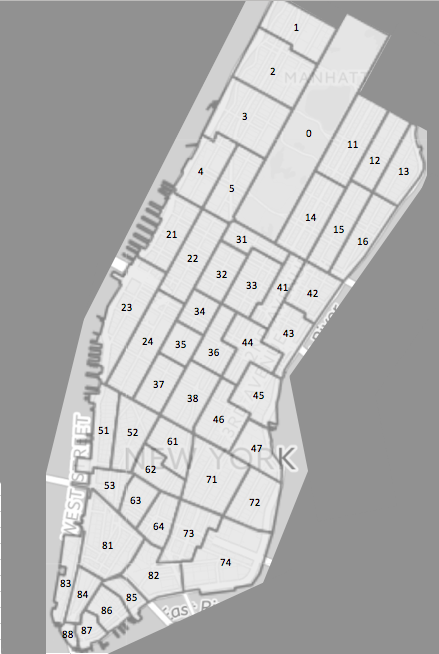
\includegraphics[width=8cm]{Figures/Manhattan.png}
\end{figure}

\indent Regarding hour, I set 5 hours (from hour 18 to 22, on the pick-up time basis) as a single unit firstly because these hours are peak hours and thus most medallions are working\footnote{I don't have a panel identifier as Frechette et al. (2016) did, so I don't have precise information how many medallions are working for each location at a specific hour. Therefore, I choose to use only peak hours in order to minimize errors in the number of medallions.} and secondly because trips are very similar during those hours within a day and the fact contributes to thickening the number of trips with fewer errors. Figure \ref{fig:July_2012} shows the average number of daily trips of a typical month (July 2012).\footnote{The trough before the peak time is considered due to the supply side when many leased cabs end day-shifts. This is known as the "witching hour."} The number of pickups is diverge depending on the locations. While there are about 5,000 daily pickups during the 5 hours near Rockefeller Center (Location 33), there is almost no pickup at North Cove Marina\footnote{Second worst is Battery Park (Location 88) with only 30 daily pickups.} (Location 83).

\begin{figure}[h]
\centering
\caption{Number of Pickups in Manhattan}\label{fig:July_2012}\\
\vspace{0.2cm}
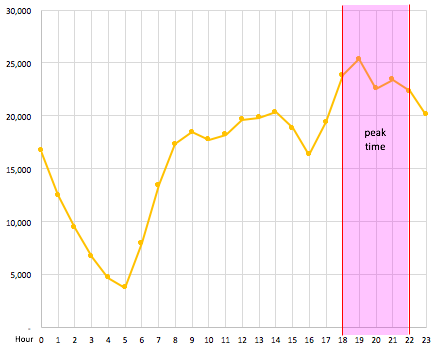
\includegraphics[width=12cm]{Figures/July_2012.png}
\end{figure}

\indent I set the number of medallions in Manhattan 8,000. This number comes from the fact that more than 70\% taxis are working during the peak hours\footnote{Source: Frechette et al. (2016)} and about 88\% of trips depart in Manhattan (yellow cab zone) during the peak time on weekdays. As the number of medallions is 13,437 (as of 2013), I set it 8,000 (\approx 13,437 \times 0.7 \times 0.88).\footnote{I checked that result is only slightly changed if I alternate it with 7,000 or 9,000. See Appendix C.} 

In this study, I don't take into consideration the unique characteristics of taxis that several passengers can share their trips and split the bill. According to the data, approximately two-thirds of trips are solo and the average number of passengers per trip is 1.73. Comparing the number of passengers per trip before and after the price increase, the distribution almost didn't change and therefore it would be no problem not to consider the number of passengers per trip in the following analyses. 

\indent Road length ranges from 1.5 miles (Battery Park, Location 88) to 16.0 miles (Lower East Side, Location 74). As each road has 2 directions, I multiply it by 2 to use as $L_i$.\footnote{I therefore assume that passengers don't pick up taxis on the other side even if vacant. See Appendix B for the road length of each location. Source: Google Map.} Using weekday data of July 2012, velocity is mainly between 9 and 18 miles per hour depending on the locations and days in Manhattan, and the traffic is often slow in Midtown (Location 30's) and Little Italy (Location 60's). On the other hand, the velocity of trips outside Manhattan is between 17 and 20 mph and relatively stable. Average trip time is 9.7 minutes. These statistics are summarized in Table \ref{tab:summary_statistics}.\footnote{Summary of data from hour 18 to 22 (based on pickup time) in July 2012}

\begin{table}[h]
\caption{Summary of the Statistics}\label{tab:summary_statistics}\\

{
\def\sym#1{\ifmmode^{#1}\else\(^{#1}\)\fi}
\begin{center}
\begin{tabular}{l*{5}{c}}
\hline\hline
            
            &\multicolumn{1}{c}{{Mean}}&\multicolumn{1}{c}{S.D.}&\multicolumn{1}{c}{25 \%ile}&\multicolumn{1}{c}{Median}&\multicolumn{1}{c}{75 \%ile}\\
\hline
Fare (\$)* & 7.75 & 3.77 & 5.30  & 6.90 & 9.30\\
Distance (mile) & 1.84  & 1.37 & 0.99 & 1.50 & 2.30\\
Trip Time (min.) & 9.66 & 5.76 & 6 & 9 & 12\\
Number of Daily Trips inside Manhattan & 92,836  & 13,845 & 84,532 & 94,815 & 105,123  \\
Velocity (Inside Manhattan, mph) & 11.85 & 4.69 & 8.80 & 11.33 & 14.25\\
Velocity (Outside Manhattan, mph) & 18.95 & 1.12 & 18.20 & 18.73 & 20.11\\
Wait Time (min.) & 1.94 & 3.09 & 0.67 & 1.02 & 1.75\\
Search Time (min.) & 9.64 & 4.37 & 6.40 & 8.78 & 12.20\\

\hline\hline
\end{tabular}
\end{center}
}

{\hspace{1cm}\footnotesize *Fare composes of base fare, distance fare/time charge. Miscellaneous surcharges are omitted.}\\

\end{table}




\indent From these numbers, search time, wait time and the number of waiting passengers can be calculated. Search time is 9.6 minutes on average (median is 8.8 minutes) and wait time is 1.9 minutes on average (median is 1.0 minute).\footnote{Statistics of wait time and search time are not weighted by the number of trips, so the number of observations is 50 (locations) $\times$ 31 (days) less missing/omitted ones. Fare, distance and trip time are weighted and the number of observation is 2,877,906.} Most of the search time range from 4 minutes to 18 minutes, while wait time mainly from less than 1 minute to 6 minutes. Regarding the number of passengers, using the average fastest speed ($v^H$, which is at hour 5 and approximately 20 mph), it's just less than 1\% higher than the actual trips. This would be reasonable considering that the average wait time is as short as 1.9 minutes and more than half of yellow cabs are vacant.\footnote{Rough calculation shows that each cab has passengers for $\frac{9.66 \, (average \,\, trip \,\, minutes) \times 18,567 \, (average \,\, hourly \,\, trips) }{8,000 \,(number \,\, of \,\, medallions)}$ =22.4 minutes per hour on average during the peak hours.}

\vspace{0.5cm}
\subsubsection{Demand Curve Estimation}
\hspace{0.5cm} I estimate how price and also wait time affect the number of passengers using data of June and July in 2012 and 2013. TLC raised fare in September 2012 and thus 2012 is the year before the fare increase while 2013 is after that.\footnote{$P_{ij}$ is the average of each trip's fare between location i and j. Since price is determined outside the market, there is no concern of division bias.} I use data of June and July so that passengers have enough time to recognize the fare increase and I avoid data of August as boro taxis are introduced in August 2013. Though they can't operate in yellow cab zones, this emergence would have influenced yellow cab driver's supply in Manhattan, which I assume is fixed constant. Furthermore, as there is a clear difference regarding trips trend between weekdays and weekends, I choose to use only weekdays (Monday through Thursday).\footnote{This is the same strategy as Frechette et al. (2016)} There are 69 weekdays during the 4 months and 2,500 combinations of routes, but there are many routes where there were no trips on some days, so the actual number of observations is 54,947.\footnote{I also omitted unrealistic observations where wait time is negative or longer than 20 minutes. These consist only 1.5\%.} Though fare is determined exogenously, as wait time is a result of high demand and also can be a cause of low demand, there is a problem of endogeneity and thus I implement instrument variable approach as stated in 4.1.2. 

In Equation (\ref{eq:demand_curve}), $\mathbf{\bm{\gamma} X_{ijh}}$ are velocity inside Manhattan, distance between location i and j, dummy variables of days, weather (if it rained for more than or equal to 2 hours during the peak hours\footnote{Source: Network for Environment and Weather Applications, Cornell University http://newa.cornell.edu}), clustered pickup and dropoff areas (Upper West Side, Upper East Side, Hell's Kitchen, Midtown, Midtown East, Greenwich Village, Little Italy, East Village and Lower Manhattan). Dummy variables of pickup/dropoff at Central Park are omitted to avoid exact collinearity.

\begin{table}[h]
\caption{Elasticity of Demand w.r.t Own Price and Wait Time}\label{tab:lnfare_regression}\\

{
\def\sym#1{\ifmmode^{#1}\else\(^{#1}\)\fi}
\begin{center}
\begin{tabular}{l*{2}{c}}
\hline\hline
            &\multicolumn{1}{c}{(1)}&\multicolumn{1}{c}{(2)}\\
            &\multicolumn{1}{c}{\textit{log (Waiting Passengers)}}&\multicolumn{1}{c}{\textit{log (Waiting Passengers)}}\\
\hline
\textit{log (Price)}      &      -0.437\sym{***}&      -0.386\sym{***}\\
            &    (0.0686)         &    (0.0686)         \\
[1em]
${\widehat{log\, (Wait\, Time)}}$&      -0.146\sym{*} &     -0.0943  \\
            &    (0.0662)         &    (0.0659)         \\
\hline
\(N\)       &       54,947         &       54,947         \\
\(R^{2}\)   &       0.207         &       0.214         \\
Public Transportation Effect &       No            &    Yes                 \\
\hline\hline
\multicolumn{3}{l}{\footnotesize Standard errors in parentheses}\\
\multicolumn{3}{l}{\footnotesize \sym{*} \(p<0.05\), \sym{**} \(p<0.01\), \sym{***} \(p<0.001\)}\\
\end{tabular}
\end{center}
}


\end{table}


\begin{table}[h]
\centering
\caption{Elasticity of Demand w.r.t Own Price with Cross Terms}\label{tab:lnfare_cross_regression}
\vspace{0.2cm}
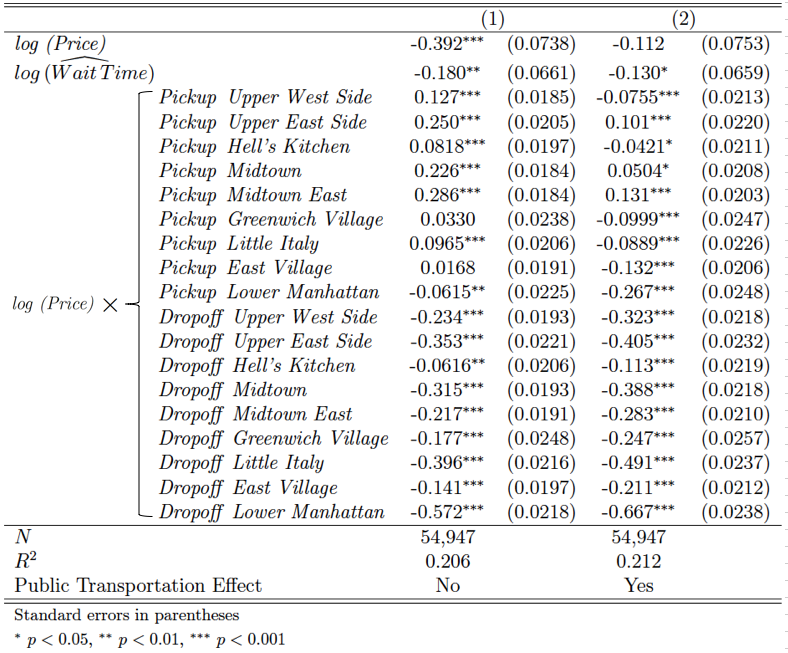
\includegraphics[width=16cm]{Tables/lnfare_cross_regression.png}
\end{table}

\begin{figure}[h]
\centering
\caption{Price Elasticities of Area-to-area Routes }\label{fig:distance_elasticity}\\
\vspace{0.2cm}
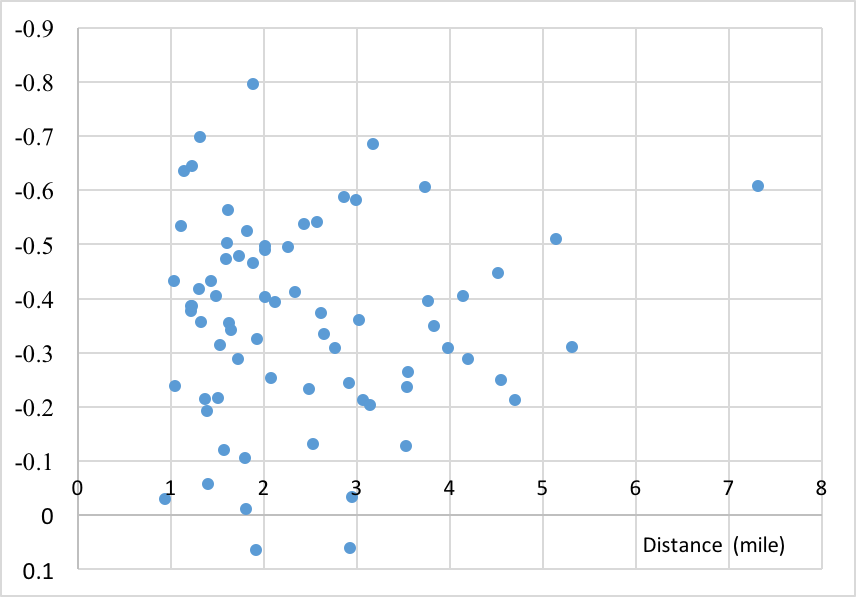
\includegraphics[width=12cm]{Figures/distance_elasticity.png}
\vspace{1.0cm}
\end{figure}


\indent $log(w_{i})$ is instrumented by velocity outside Manhattan and the coefficient is significantly negative as expected in 4.1.2. I control public transportation effects in another regression, where I additionally include in $\mathbf{\bm{\gamma} X_{ijh}}$ such variables as whether there are subway stations in pickup locations, whether there are subway stations in dropoff locations, whether it is possible to move by subway without changing trains, and whether the origins/destinations are close to Penn/Grand Central stations. This additional regression reflects the idea that outside options would be different for different routes.



\indent Table \ref{tab:lnfare_regression} shows the regression results. Both of the elasticities of demand with respect to price and wait time are significant when public transportation effect is not taken into consideration. Once controlled for the effect, wait time becomes insignificantly different from 0 but the sign is still negative as expected. Controlling for transportation slightly lowers the estimations of the elasticities. Demand is price inelastic and this is intuitive as yellow cabs are often used as important transportation in Manhattan and there was no close substitute like Uber at that time. Regarding wait time, it is very inelastic and this might reflect the simulation result that wait time is shorter than 2 minutes in most cases and thus few people would have given up finding vacant cabs.

\indent I also checked whether the price elasticity is dependent on distance, as the percentage of price increase is higher for longer trips. Dummy variables of pickup and dropoff areas in $\mathbf{\bm{\gamma} X_{ijh}}$ above are replaced by the cross terms of "$log (Price)$ $\times$ pickup/dropoff areas" and regressions are exercised in the same way. The result is in Table \ref{tab:lnfare_cross_regression}. Coefficients of the cross terms are also displayed. In this case, $log (Price)$ is price elasticity of the route which passengers are both picked up and dropped off within the area of the central park. Depending on the pickup/dropoff areas there are some variations of price elasticities. See Appendix D for the variance-covariance matrix of the variables and the estimated elasticity for each pickup/dropoff area, which are calculated using the regression result with public transportation effect.

Figure \ref{fig:distance_elasticity} shows the results of price elasticities of area-to-area routes using the regression result with public transportation effects in Table \ref{tab:lnfare_cross_regression} (or Table \ref{tab:each_lnfare}).\footnote{As some area-to-area routes have no trips, the number of points on the figure is less than 100.} Horizontal axis is distance and calculated by taking the mean of the distance of trips between (or within) areas. The result is that though price elasticities somewhat depend on origins/destinations of the routes and are mostly between 0.1 and 0.9, the figure suggests that they are not dependent on distance. Correlation is -0.02 and is not statistically significantly different from 0. This evidence supports that the demand for taxis is inelastic for the fare increase by various percentage. 

\vspace{0.5cm}



\subsection{Welfare Analysis of Price Increase}
\hspace{0.5cm} Next, I calculate how consumer welfare changed before and after the price change. As the demand curve is assumed constant regarding price elasticities conditional on pickup/dropoff locations, even if the price is extremely high, there are few but some passengers who are still willing to pay and thus consumer welfare calculated by simple integration becomes arbitrarily large. Therefore, I instead calculate the lower bound\footnote{Similar approach is adopted in Buchholz (2016)} of consumer surplus for each year by summing every area-to-area route as in the Equation (\ref{eq:consumer_surplus}).


\begin{equation}
Consumer\,\, Surplus = \sum_k \sum_l \frac{1}{2}(P^H_{kl}-\overline{P_{kl}})\overline{Q^d_{kl}}\label{eq:consumer_surplus}
\end{equation}

\noindent , where k/l are 10 pickup/dropoff areas and $P^H_{kl}$ is the hypothetical highest price passengers would pay for the route from area k to l (explained later), while $\overline{P_{kl}}$ is an average price and $\overline{Q^d_{kl}}$ is the number of waiting passengers, both of which are realized in equilibrium. The image of the consumer surplus is in Figure \ref{fig:welfare_price}. All of the variables are indexed by kl but are omitted in the figure for ease of reading. 

\begin{figure}[h]
\centering
\caption{Consumer Surplus by Trips from k to l}\label{fig:welfare_price}\\
\vspace{0.2cm}
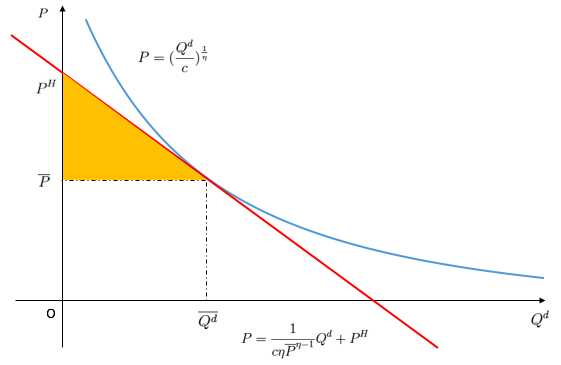
\includegraphics[width=12cm]{Figures/welfare_price.png}
\vspace{1.0cm}
\end{figure}


The blue curve is the estimated demand curve. Taking exponential of the both sides of Equation (\ref{eq:demand_curve}), and denoting other variables than price $c_{kl}$, the demand curve can be written as $Q^d_{kl}= c_{kl}P_{kl}^{\eta_{kl}}$, where $\eta_{kl}$ is the price elasticity of trips from k to l and can be calculated from Table \ref{tab:lnfare_cross_regression} (or Table \ref{tab:each_lnfare}). Solving for $P_{kl}$, the equation written in the figure is obtained. Taking the derivative of the demand curve with respect to $P_{kl}$ at the realized price $\overline{P_{kl}}$, the red tangent line is calculated as in the figure. $P^H_{kl}$ is the intercept with the tangent line and the lower bound of the consumer surplus is the surface of the orange triangle.

The result is in Table \ref{tab:welfare_price}. As the number of weekdays (Monday through Thursday) are different between June/July in 2012 and 2013, the consumer surplus during peak hours is shown on a daily basis. It declined from 5.32 million dollars to 5.00 million dollars, or decreased by 6.0\%, and the main cause would be the price increase.\footnote{Note that the consumer surplus is the lower bound and considering also that the standard errors of the elasticities are relatively large, the result is just suggestive.}

\begin{table}[h]
\caption{Comparison of Surplus}\label{tab:welfare_price}\\

{
\def\sym#1{\ifmmode^{#1}\else\(^{#1}\)\fi}
\begin{center}
\begin{tabular}{l*{5}{c}}
\hline\hline
Year & Daily Consumer Surplus & Daily Producer Surplus & Total\\
\hline
 2012 & \$ 5.32 M & \$ 0.26 M & \$ 5.58 M\\
 2013 & \$ 5.00 M & \$ 0.38 M & \$ 5.38 M\\

 
 


\hline\hline
\end{tabular}
\end{center}
}


\end{table}


Producer surplus can also be measured by back-of-the-envelope calculation. I here define the producer surplus as gross fare revenue\footnote{Miscellaneous surcharges are excluded as they don't go to drivers.} minus fuel and lease cost.\footnote{Thus I simplify that all of the medallions are leased.} Average daily fare during peak time is \$ 776,000 and \$ 889,000 in 2012 and 2013 respectively. According to TLC Factbook 2014, average fuel economy is 29 miles per gallon, and the gas price is \$3.602 per gallon on average in 2013, and the lease rate cap for night-shift (at least for 9 hours) is between \$115 to \$129.\footnote{Lease rate cap depends on day/night shift and day. \\See http://www.nyc.gov/html/tlc/downloads/pdf/fleet\_drivers\_rights\_poster.pdf } From these data, combined with the number of medallions and average velocity, daily consumer surplus during peak time is roughly calculated as \$264,000 and \$377,000 dollars in 2012 and 2013 respectively. Though price increase brought about higher producer surplus, the rise didn't compensate the loss of consumer surplus, leading to the smaller total surplus.